\documentclass[a4paper,12pt]{article}
	
\usepackage[T2A]{fontenc}			
\usepackage[utf8]{inputenc}			
\usepackage[english,russian]{babel}	

\usepackage[
bookmarks=true, colorlinks=true, unicode=true,
urlcolor=black,linkcolor=black, anchorcolor=black,
citecolor=black, menucolor=black, filecolor=black,
]{hyperref}

\usepackage{color}
\usepackage{caption}


\usepackage{amsmath,amsfonts,amssymb,amsthm,mathtools} 
\usepackage{wasysym}

\usepackage{graphicx}
%\usepackage[cache=false]{minted}
\usepackage{cmap}
\usepackage{indentfirst}

\usepackage{listings} 
\usepackage{fancyvrb}
\usepackage{slashbox}

\usepackage{geometry}
\geometry{left=2cm}
\geometry{right=1.5cm}
\geometry{top=1cm}
\geometry{bottom=2cm}

\setlength{\parindent}{5ex}
\setlength{\parskip}{0.5em}

\usepackage{titlesec}
\usepackage{pgfplots}
\usepackage{filecontents}
\usetikzlibrary{datavisualization}
\usetikzlibrary{datavisualization.formats.functions}

\DeclareCaptionFont{white}{\color{white}}
\DeclareCaptionFormat{listing}{\colorbox{gray}{\parbox{\textwidth}{#1#2#3}}}
\captionsetup[lstlisting]{format=listing,labelfont=white,textfont=white}
\lstloadlanguages{% Check Dokumentation for further languages ...
C,
C++,
csh,
Java
}

\definecolor{red}{rgb}{0.6,0,0} % for strings
\definecolor{blue}{rgb}{0,0,0.6}
\definecolor{green}{rgb}{0,0.8,0}
\definecolor{cyan}{rgb}{0.0,0.6,0.6}

\lstset{ %
language=Lisp,                 % выбор языка для подсветки
basicstyle=\small\sffamily, % размер и начертание шрифта для подсветки кода
numbers=left,               % где поставить нумерацию строк (слева\справа)
numberstyle=\tiny,           % размер шрифта для номеров строк
stepnumber=1,                   % размер шага между двумя номерами строк
numbersep=5pt,                % как далеко отстоят номера строк от подсвечиваемого кода
showspaces=false,
backgroundcolor=\color{white},         
showstringspaces=false,      % показывать или нет пробелы в строках
showtabs=false,             % показывать или нет табуляцию в строках
frame=single,              % рисовать рамку вокруг кода
tabsize=2,                 % размер табуляции по умолчанию равен 2 пробелам
captionpos=t,              % позиция заголовка вверху [t] или внизу [b] 
breaklines=true,           % автоматически переносить строки (да\нет)
breakatwhitespace=false, % переносить строки только если есть пробел
escapeinside={\%*}{*)}
}

% Для измененных титулов глав:
\definecolor{gray75}{gray}{0.75} % определяем цвет
\newcommand{\hsp}{\hspace{20pt}} % длина линии в 20pt
% titleformat определяет стиль
\titleformat{\chapter}[hang]{\Huge\bfseries}{\thechapter\hsp\textcolor{gray75}{|}\hsp}{0pt}{\Huge\bfseries}

\begin{document}
	
\begin{figure}[h!]
	\begin{center}
		{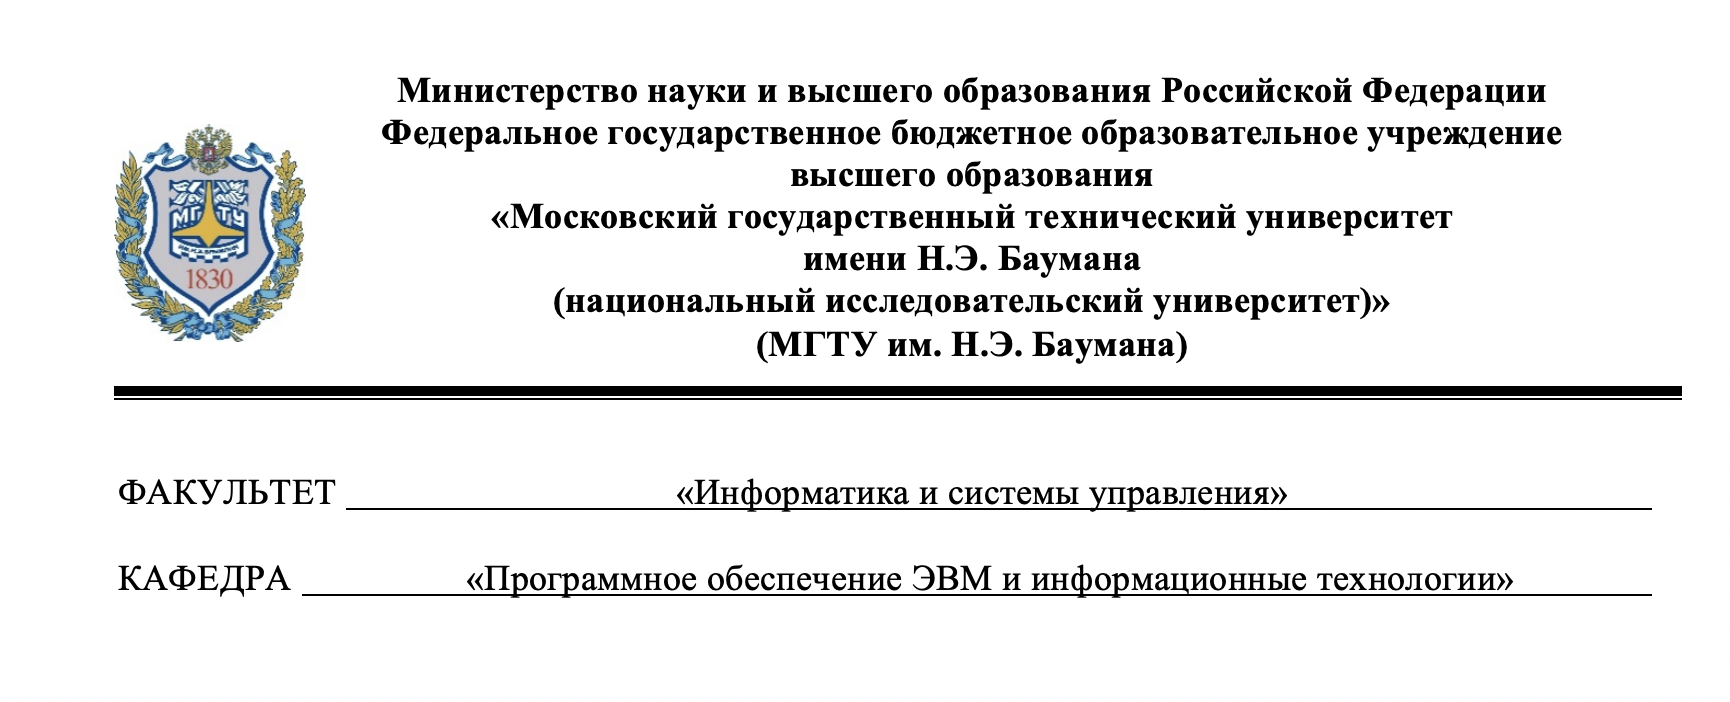
\includegraphics[width = \textwidth]{titul.png}}
	\end{center}
\end{figure}

\vspace*{20mm}

\huge
\begin{center}
	Лабораторная работа №5
\end{center}


\vspace*{50mm}

\large
\begin{flushleft}
	Студент: Луговой Д.М. \\
	Группа: ИУ7-61Б \\
	Преподаватель: Толпинская Н.Б.
\end{flushleft}

\vspace*{60mm}

\large
\begin{center}
	Москва, 2020 г.
\end{center}

\thispagestyle{empty}

\newpage
\vspace*{10mm}
\textbf{Цель работы}: приобрести навыки работы в Common Lisp.\\

\textbf{Задачи работы}: изучить работу интерпретатора Lisp, алгоритм работы функции eval, структуру и порядок обработки программы в Lisp.

\begin{enumerate}
\item \textbf{Представление атома в памяти}
Атомы - это элементарные элементы Lisp, из которых строятся остальные структуры.
Атомы в Lisp:
\begin{itemize}
\item Символы - последовательность из букв и цифр, начинающаяся с буквы, включая и другие литеры, не занятые в синтаксисе.
\item Специальные символы - логические константы T и Nil.
\item Самовычислимые атомы - натуральные, дробные и вещественные числа и строки.
\end{itemize}

В памяти атом представлен как структура из 5 указателей:
\begin{figure}[ht!]
\center{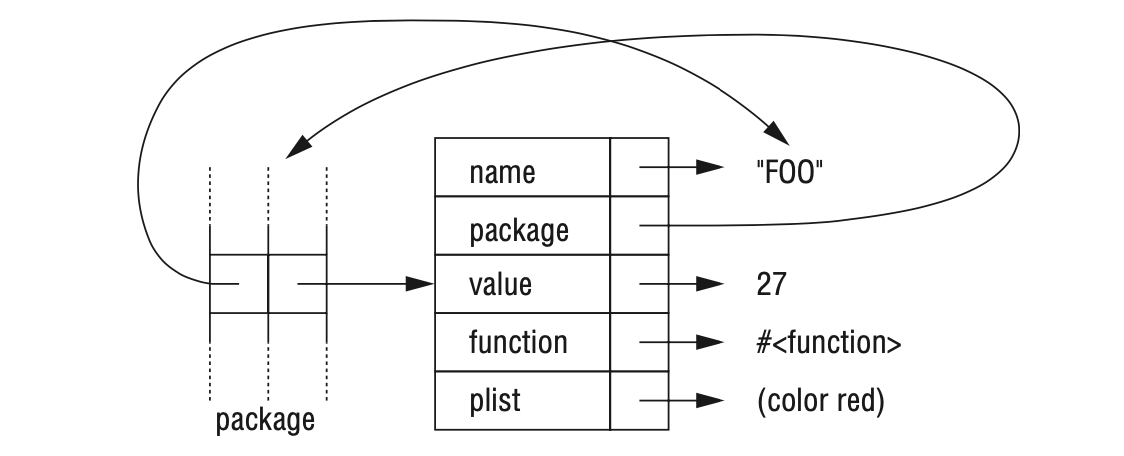
\includegraphics[scale=0.8]{FaLP2.png}}
\end{figure}

\item \textbf{Самовычисляемые атомы}

В Lisp натуральные, дробные и вещественные числа и строки, а также константы Nil и T являются самовычисляемыми.
Это означает, что когда данный объект вычисляется, он (или возможно копия в случае с числами и строковыми символами) возвращается в качестве значения.

Например, при вычислении атомов 10 или "Hello, world!"  эти атомы будут вычислены в 10 и "Hello, world!" соответсвенно.

\item \textbf{Локальное и глобальное определение значения атома}

Локальные значение атома можно определить с помощью функций let и let*. Областью видимости является тело функции, в которой определена переменная.

Синтаксис:

(let ((var1 value1) (var2 value2) ... (varN valueN)) body)

Сначала вычисляются значения value1, value2, ... , valueN, а затем происходит их связывание с var1, var2, ... , varN. 

(let* ((var1 value1) (var2 value2) ... (varN valueN)) body)

Отличие от let состоит в том, что связывание каждого значения value с символом var происходит сразу после вычисления значения.

Глобальные значение атома устанавливается с помощью функции setf. Областью видимости является весь код, следующий после определения.

Синтаксис: 

(setf var value)

\item \textbf{Функции EVAL и QUOTE}

Функция eval, вычисляет заданное выражение и возвращает его значение:

(eval ’(+ 1 2 3)) -> 6

Схема выполнения Eval:
\begin{figure}[ht!]
\center{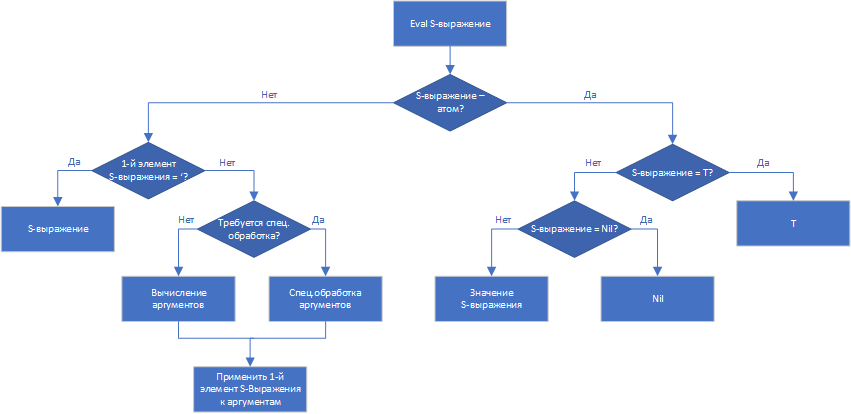
\includegraphics[scale=0.82]{FaLP1.png}}
\end{figure}
\end{enumerate}

И программа, и данные в Lisp представляются в списочной форме. Для явного выделения данных используется функция QUOTE и ' - ее сокращенное обозначение. Эта функция защищает выражение от вычисления. 

Если eval была применена явно, блокировка вычисления quote не сработает, так как eval обеспечивает дополнительный вызов интерпретатора.

\newpage
\vspace*{10mm}
{\LARGE Задание №1}\\

Написать функцию, которая принимает целое число и возвращает первое четное число, не меньшее аргумента.

(defun get\_even (x) (cond ((oddp x)(+ x 1)) (x)))

Примеры:
\begin{itemize}
\item (get\_even 4) -> 4
\item (get\_even 7) -> 8\\
\end{itemize}

{\LARGE Задание №2}\\

Написать функцию, которая принимает число и возвращает число того же знака, но с модулем на 1 больше модуля аргумента.

(defun inc\_abs (x) (cond ((plusp x)(+ x 1))((- x 1))))

Примеры:
\begin{itemize}
\item (inc\_abs 3) -> 4
\item (inc\_abs -5) -> -6\\
\end{itemize}

{\LARGE Задание №3}\\

Написать функцию, которая принимает два числа и возвращает список из этих чисел, расположенный по возрастанию.

 (defun get\_asc (x y) (cond ((> x y)(list y x))((list x y))))

Примеры:
\begin{itemize}
\item (get\_asc 3 5) -> (3 5)
\item (get\_asc 5 -1) -> (-1 5)\\
\end{itemize}

\newpage
\vspace*{10mm}
{\LARGE Задание №4}\\

Написать функцию, которая принимает три числа и возвращает T только тогда, когда первое число расположенно между вторым и третьим.

(defun between (a b c) (or (and (> a b) (< a c)) (and (< a b) (> a c))))

Примеры:
\begin{itemize}
\item (between 8 7 10) -> T
\item (between 2 3 0) -> T
\item (between 1 5 8) -> NIL\\
\end{itemize}

{\LARGE Задание №5}\\

Каков результат вычисления следующих выражений?

\begin{enumerate}
\item (and 'fee 'fie 'foe)\\
Результат: FOE
\item (or 'fee 'fie 'foe)\\
Результат: FEE
\item (and (equal 'abc 'abc) 'yes)\\
Результат: YES
\item (or nil 'fie 'foe)\\
Результат: FIE
\item (and nil 'fie 'foe)\\
Результат: NIL
\item (or (equal 'abc 'abc) 'yes)\\
Результат: T\\
\end{enumerate}

\newpage
\vspace*{10mm}
{\LARGE Задание №6}\\

Написать предикат, который принимает два числа-аргумента и возвращает Т, если первое число не меньше второго.

(defun is\_greater (x y) (>= x y))

Примеры:
\begin{itemize}
\item (is\_greater 5 2) -> T
\item (is\_greater 7 20) -> NIL
\item (is\_greater 6 6) -> T\\
\end{itemize}

{\LARGE Задание №7}\\

Какой из следующих двух вариантов предикатов ошибочен и почему?

\begin{enumerate}
\item (defun pred1 (x) (and (numberp x) (plusp x)))
\item (defun pred2 (x) (and (plusp x) (numberp x)))
\end{enumerate} 

Ошибочен второй предикат, так как в нем сначала вычисляется предикат plusp, который может вернуть ошибку в случае, если x не является числом, а первый предикат в этом случает вычислит предикат numberp, вернет NIL и предикат plusp вычислен не будет.\\

{\LARGE Задание №8}\\

Решить задачу 4, используя для ее решения конструкции:
\begin{itemize}
\item COND\\
(defun between (a b c) (cond ((cond ((> a b) (< a c)) ((< a b) (> a c))))))
\item IF\\
(defun between (a b c) (if (> a b) (< a c) (if (< a b) (> a c))))
\item AND/OR\\
(defun between (a b c) (or (and (> a b) (< a c)) (and (< a b) (> a c))))
\end{itemize}
\end{document}